%zusammenfassung

%gegenseitige beeinflussung: showrooming-effekt: kauf online aufgrund von stationärere beratung -- kauf stationär nach onlinerecherche \cite[S. 21f]{evilcom}

%wie viele läden haben in schleusingen einen onlineshop?


\begin{folding} %stationärer Handel

Aufgrund der Verschiebung von Nachfrage und Bedürfnissen von Konsumenten in den letzten Jahrzehnten wird der stationäre Handel trotz Multichannel-Versuchen keine einfache Zukunft haben. So kann in vielen Fällen stattdessen direkt von Herstellern gekauft werden, die mittlerweile den Vertriebswegwechsel von \ac{B2B} zu \ac{B2C} weitesgehend hinter sich haben. 
Insbesondere in Thüringen steht es im Vergelich zum Rest Deutschlands dank der Kombination aus schlechter Kaufkraft und niedriger Bevölkerungszahl pro Fläche schlecht um den konventionellen Einzelhandel\cite[S. 29]{Nitt}. Dazu kommen demografische Änderungen, die insbesondere in der Mitte Deutschlands Probleme verursachen: so nimmt die Bevölkerung z. B. in Hamburg, trotz Schrumpfen der Bevölkerungszahl, zu - jedoch nicht in Hildburghausen, einer der Landkreise, die am meisten Bewohner verliert\cite[S. 32f]{Nitt}. 
Zum Glück einiger Vertriebe treffen diese schlechten Chancen nicht auf alle Branchen zu - der Lebensmittelvertrieb hat z. B. kaum Online-Konkurrenz[Umfrage]. Um in den restlichen Geschäftssektoren einen maximale großen Umsatz zu erzielen, sollte der konventionelle Einzelhandel aufgrund der alternden Bevölkerung, die meist noch stationär kauft, vorerst Investitionen für die wachsende Gruppe von Senioren und dementsprechend Erreichbarkeit o. ä. nutzen.

\end{folding}

\begin{folding} \subsubsection{Der Umwelt-Aspekt} %Umweltverschmutzung

Zudem kommt immer öfter das Argument auf, dass der Wechsel zum Onlinehandel umweltschädlich sei, da mehr Lieferfahrzeuge unterwegs sind. Jedoch haben bereits die Autoren des "Evil Commerce [...]"-Buches diese These anhand einer Modellrechnung weitesgehend wiederlegt. Sie berechneten eine 90\%-ige Kraftstoffersparniss bei komplettem Umstieg zum Distanzhandel in Großstädten unter optimalen Bedingungen\cite[S. 25f]{evilcom}. Um genauerer Aussagen bezüglich des ländlichen Raumes zu treffen, werde ich die genannte Rechnung bzgl. Entfernung - da Einkaufszentren nicht berücksichtigt wurden - modifizieren und insofern erweitern, dass zusätzlich ein Einkauf in mehreren Geschäften nacheinander mit in Betracht gezogen wird.

\begin{itemize}

\item Im meiner Modellrechnung kaufen 100 Bewohner eines Dorfes in einer 4km entfernten Stadt ein. Sie kaufen im Durchschnitt in 3 von 10 Einkaufsmöglichkeiten ein, die je 500m voneinander entfernt sind. Dabei gehe ich davon aus, dass alle Kunden über eine 500m lange Straße innerhalb des Dorfes zu erreichen sind.

\item Wenn alle Bewohner stationär kaufen, legen sie im Durchschnitt eine Strecke von 

\begin{align}(250m + 4000m + 3 \cdot 500m + 4000m + 250m) \cdot 100 = 1000000m\end{align}

 zurück. Dabei nehme ich an, dass alle Bewohner denselben Ortsausgang benutzen und somit einen durchschnittlichen Weg von 250m zu diesem besitzen.

\item Wenn jeder Verkäufer jedoch die Güter an seine im Durchschnitt 30 Kunden versendet, müssten alle Lieferwagen zusammen eine Strecke von gerade einmal 

\begin{align}(4000m + 500m + 4000m) \cdot 10 = 85000m\end{align}

zurücklegen.
\item In dieser Darstellung hat der Distanzhandel eine ähnlich hohe Kraftstoffersparniss - 91.5\%. 

\end{itemize}
Zwar kann mithilfe dieses Modelles die These der Umweltverschmutzung auch auf dem Land im Allgemeinen wiederlegt werden, jedoch ist sie keine genaue Darstsellung der Realität, da viele Faktoren, wie z. B. die Retouranzahl, die beispielsweise in der Modebranche überproportional hoch ist, nicht beachtet wurden(ebd.). Außerdem beschreibt diese Rechnung ein System der Güterbeschaffung, die aussschließlich über den Versandhandel stattfindet. Jedoch wird dieses mit hoher Wahrscheinlichkeit nicht einmal in den nächsten Jahrzehnten erreicht werden - manche Produkte können nicht durch den Distanzhandel allein abgedeckt werden, zudem wird es immer Personen geben, die den analogen Beschaffungsweg bevorzugen und diesen dementsprechend wählen.

\end{folding}

\begin{folding} \subsubsection{Einfluss der Corona-Situation}
 % amazon gestärkt - einfluss auf kleine onlinehändler kaum spürbar
 
 Wie bereits in 4.1.2 angesprochen schadet die Corona-Situation dem stationären Handel, insbesondere im Einzelhandelsbereich immens. Der Onlinehandel gewinnt aufgrund von flexibleren und bequemeren Verkaufsabläufen immer mehr Kunden, auch in Bereichen, die vom Offlinehandel dominiert werden, wie den \ac{FMCG}. 
Diese machten 2019 ohne Corona-Einfluss 42.5\% der stationären Verkäufe, und gleichzeitig nur 8.4\% der Verkäufe mittels Distanzhandel aus. Insgesamt wurden gerade einmal 2.2\% der \ac{FMCG} nicht vor Ort gekauft - jedoch ist diese Zahl im Verlauf von 2020 stark gestiegen. Insbesondere bei Produkten, die mit Corona in Verbindung gebracht werden können, steigt das Online-Interesse stark, wie man an folgender Auswertung von Google-Suchanfragen erkennen kann:  

 \begin{figure}[h]
    \begin{center}
        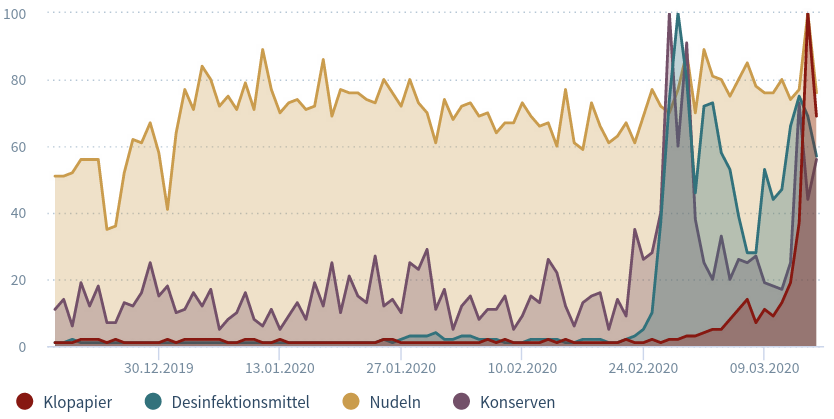
\includegraphics[width=8cm]{media/Fabian-Corona-Produkte.png}
        \caption{Onlinehandel: Die Deutschen im Krisenmodus}
        \label{konsumwandel}
        \bildquelle  Engels, Barbara:   Corona: Schub für den Onlinehandel. Version: 2020. http://hdl.handle.net/10419/215509. Köln: Institut der deutschen Wirtschaft (IW), 2020 (29/2020). – IW-Kurzbericht
    \end{center}
\end{figure}
Außerdem könnte die Angst, sich anzustecken ein weiterer Grund für den starken Nachfragezuwachs sein. Kunden, die vorerst aussschließlich stationär gekauft haben und nun erste Käufe online tätigen, können vor allem in Zukunft den Nachfrageumschwung von Offline- zu Onlinehandel noch verstärken\cite{corona-schub}.

Die immens hohe Nachfrage hat aber nicht ausschließlich positive Auswirkungen auf den Onlinehandel: eine Umfrage des Händlerbunden im März 2020 ergab, dass 52\% der befragten 412 Online-Unternehmen eine derart hohe Nachfrage erfuhren, dass diese zu Problemen führte - 15\% mussten sogar Aufträge stornieren. Als Grund ist die Logistik unwahrscheinlich, da aufgrund von einer Corona-bedingten, vergleichsweise geringen Anzahl von gewerblichen Sendungen die Branche eine geringere Auslastung als Anfang 2020 erfährt, jedoch sind personelle Probleme denkbar, insbesondere aufgrund von Corona-Regulationen\cite{haendlerbund-studie}.
 
  
 
\end{folding}
